\section*{Anexo A. Evidencias de autoría}
\addcontentsline{toc}{section}{Anexo A. Evidencias de autoría}

\subsection*{A.1. Revisión de la fuente principal}

Las siguientes capturas corresponden a la revisión del artículo técnico publicado por DoorDash Engineering \cite{wang2022iguazu}. Los fragmentos seleccionados respaldan las decisiones arquitectónicas, los resultados y las soluciones analizadas en este informe.

\begin{figure}[H]
    \centering
    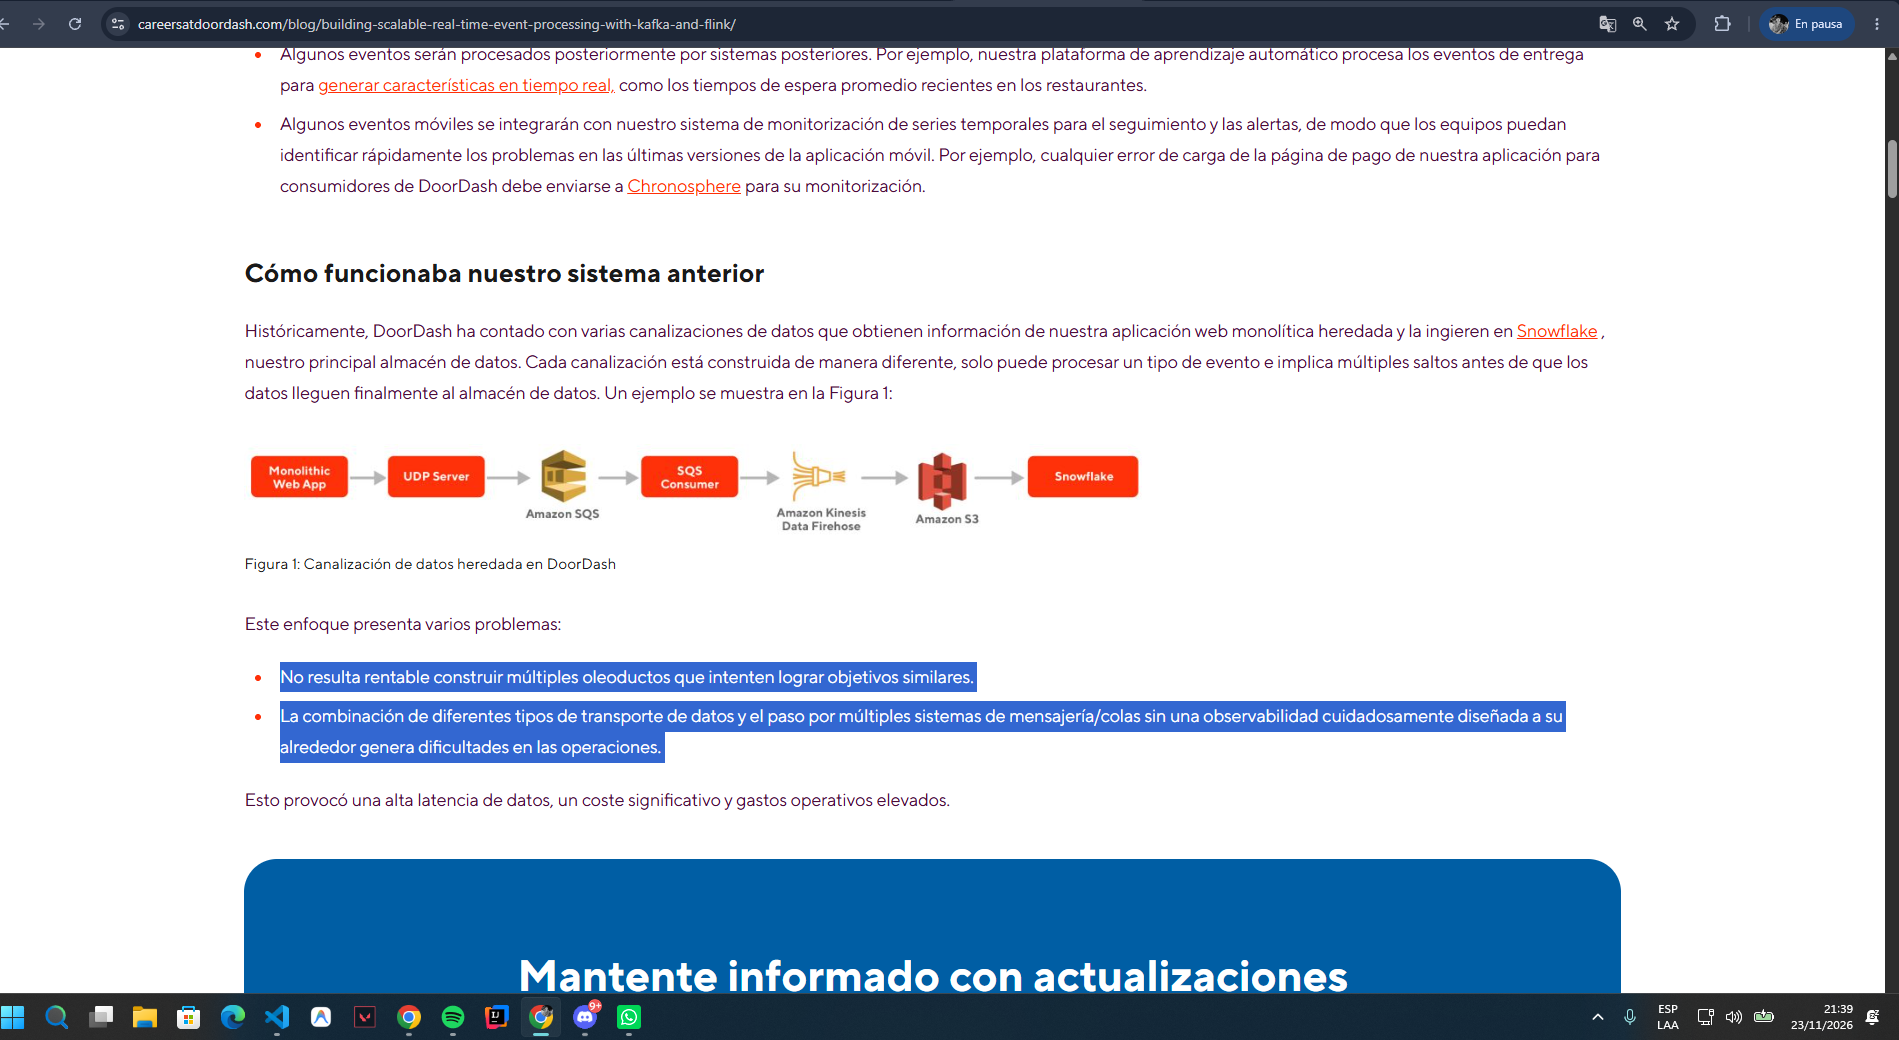
\includegraphics[width=0.95\textwidth]
    {evidencias/01_arquitectura_anterior.png}
    \caption{Limitaciones de las canalizaciones de
    datos del sistema heredado de DoorDash.}
    \label{fig:arquitectura-anterior}
\end{figure}

\begin{figure}[H]
    \centering
    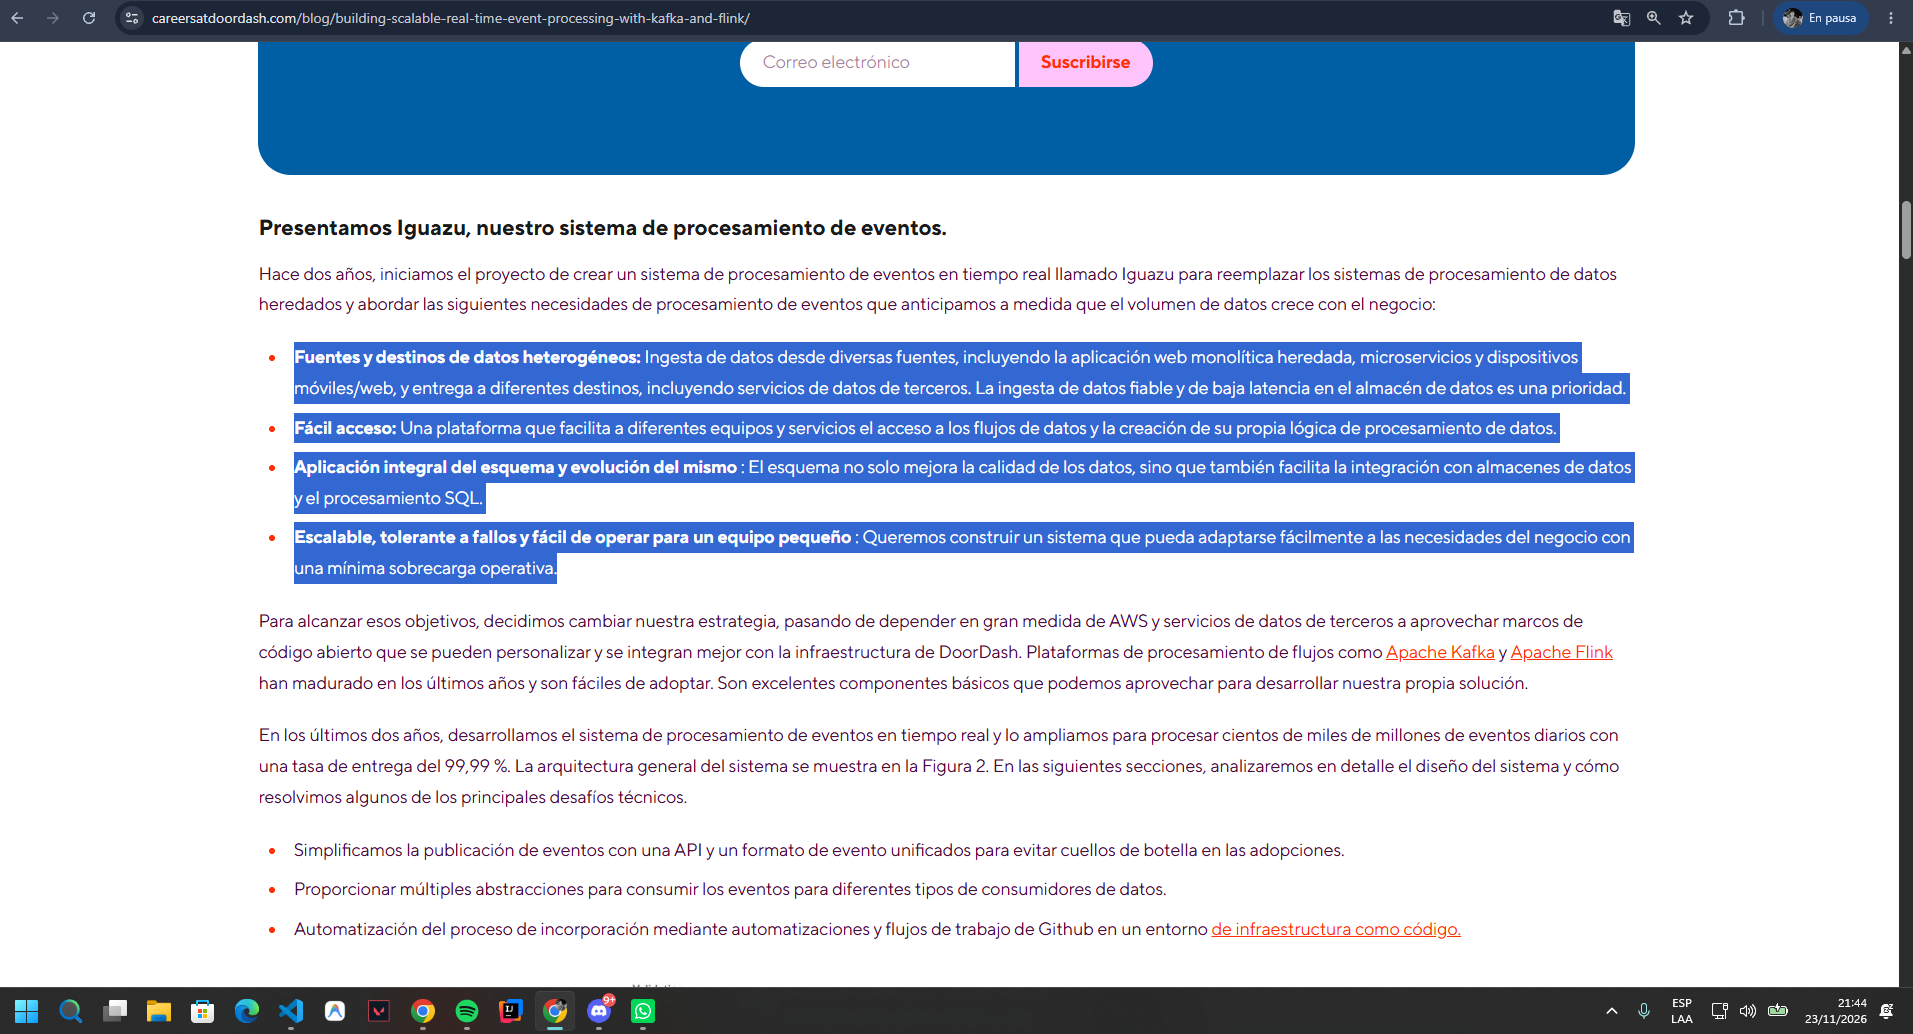
\includegraphics[width=0.95\textwidth]
    {evidencias/02_adopcion_iguazu.png}
    \caption{Necesidades que motivaron el desarrollo
    de Iguazu y la adopción de Apache Kafka
    y Apache Flink.}
    \label{fig:adopcion-iguazu}
\end{figure}

\clearpage

\begin{figure}[H]
    \centering
    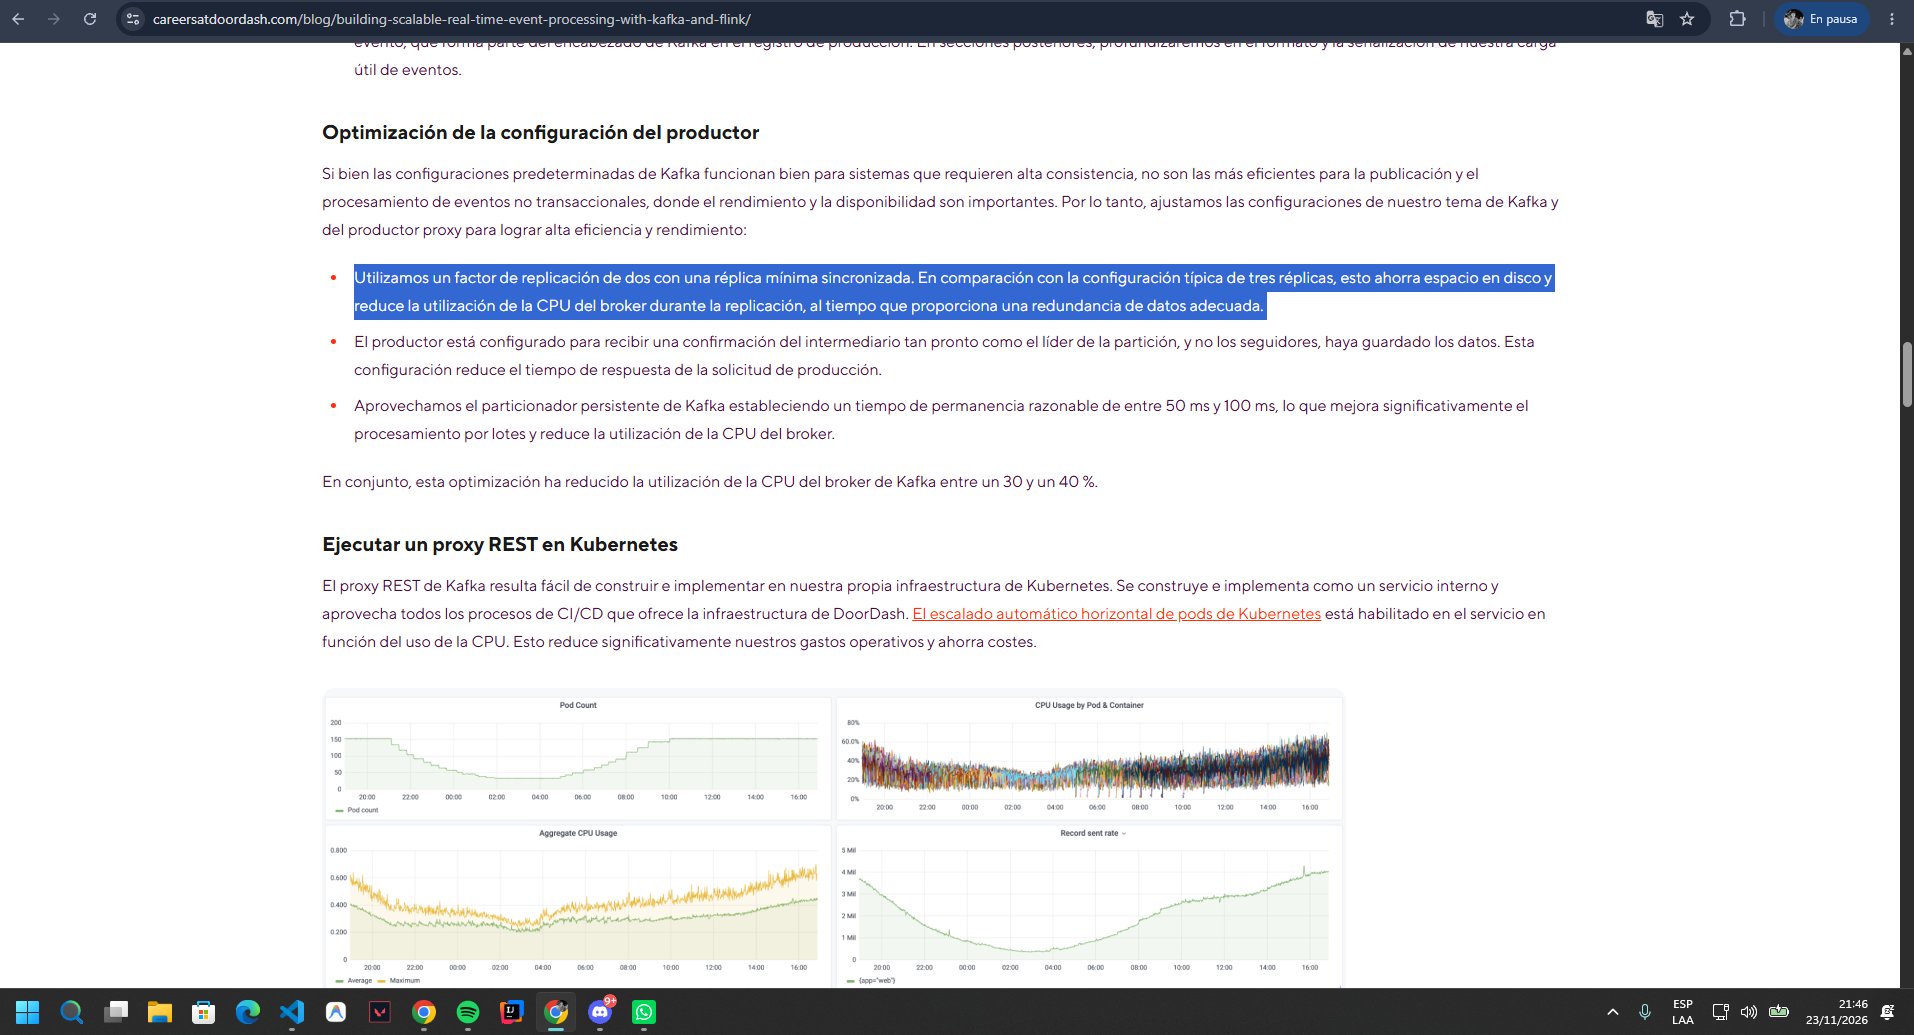
\includegraphics[width=0.95\textwidth]
    {evidencias/03_optimizacion_kafka.png}
    \caption{Optimización de la configuración del
    productor de Kafka y reducción del consumo
    de CPU.}
    \label{fig:optimizacion-kafka}
\end{figure}

\begin{figure}[H]
    \centering
    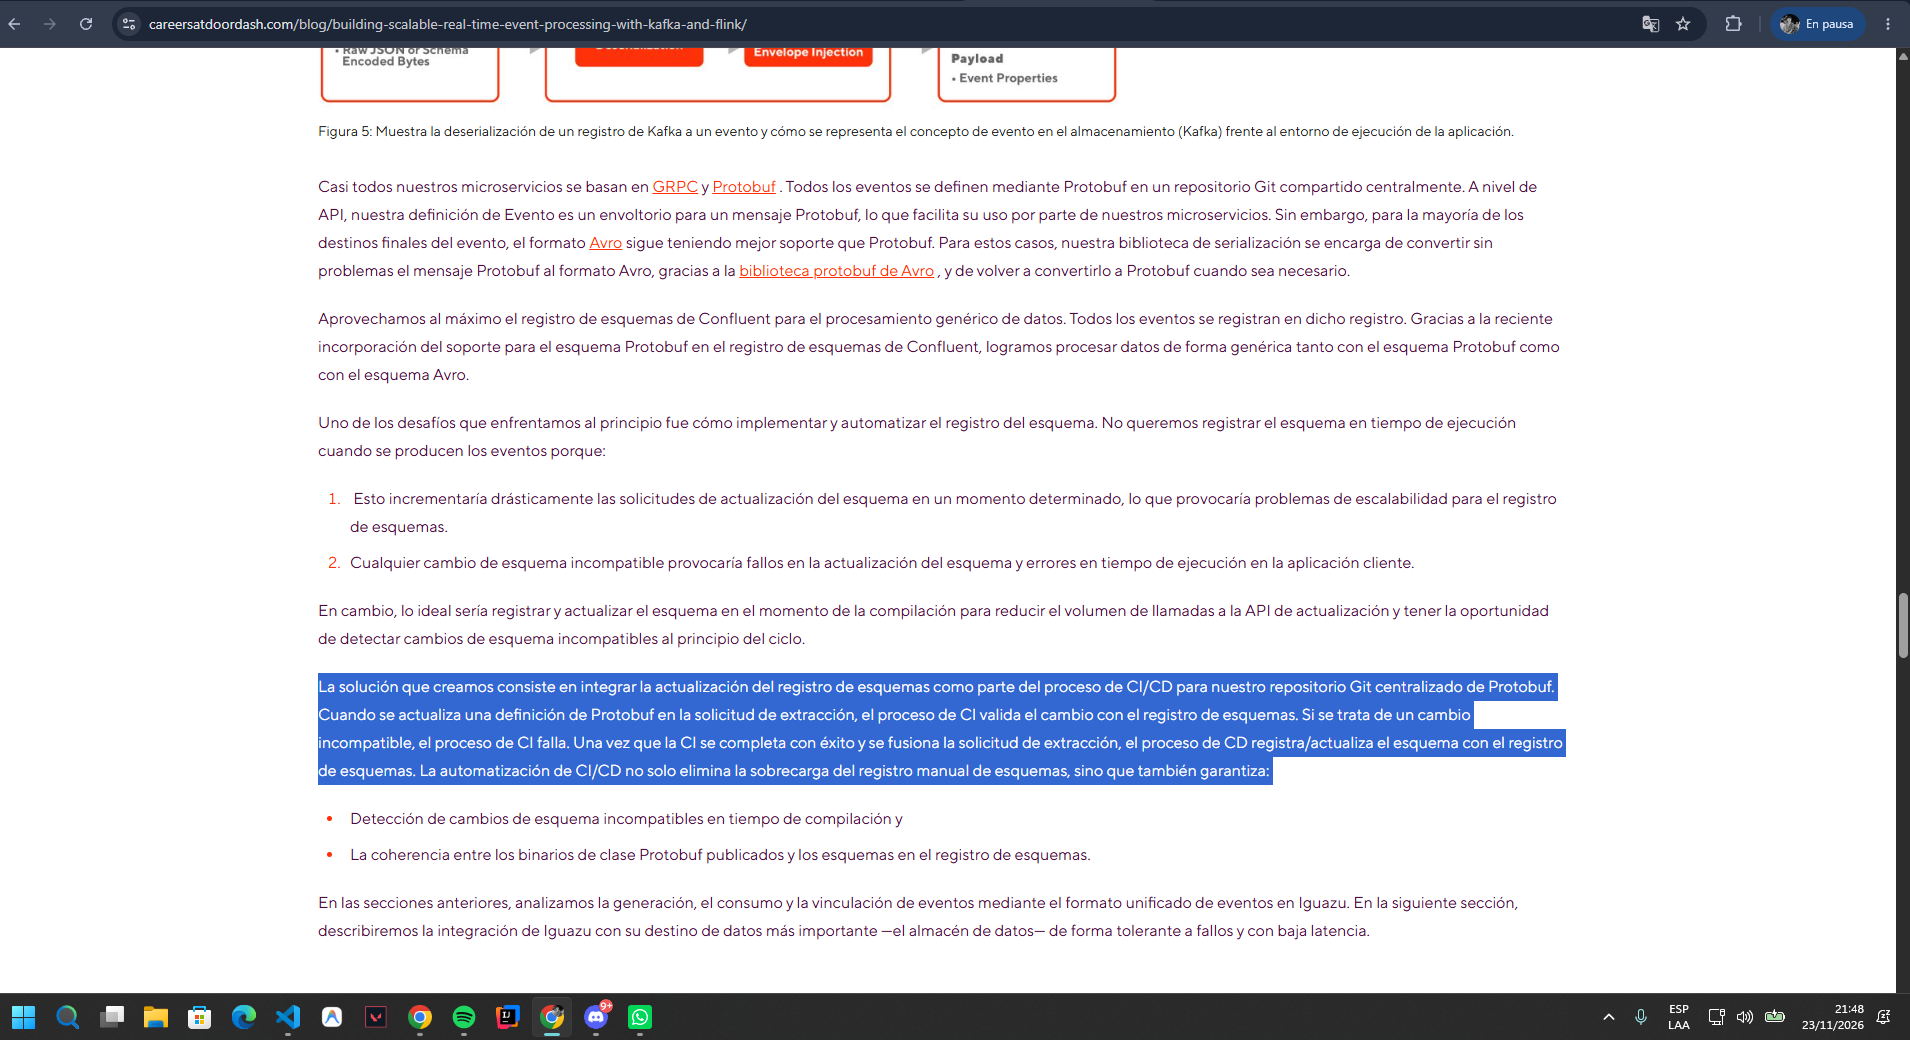
\includegraphics[width=0.95\textwidth]
    {evidencias/04_validacion_esquemas_cicd.png}
    \caption{Validación y actualización automática
    de esquemas mediante procesos de CI/CD.}
    \label{fig:validacion-esquemas}
\end{figure}

\clearpage

\begin{figure}[H]
    \centering
    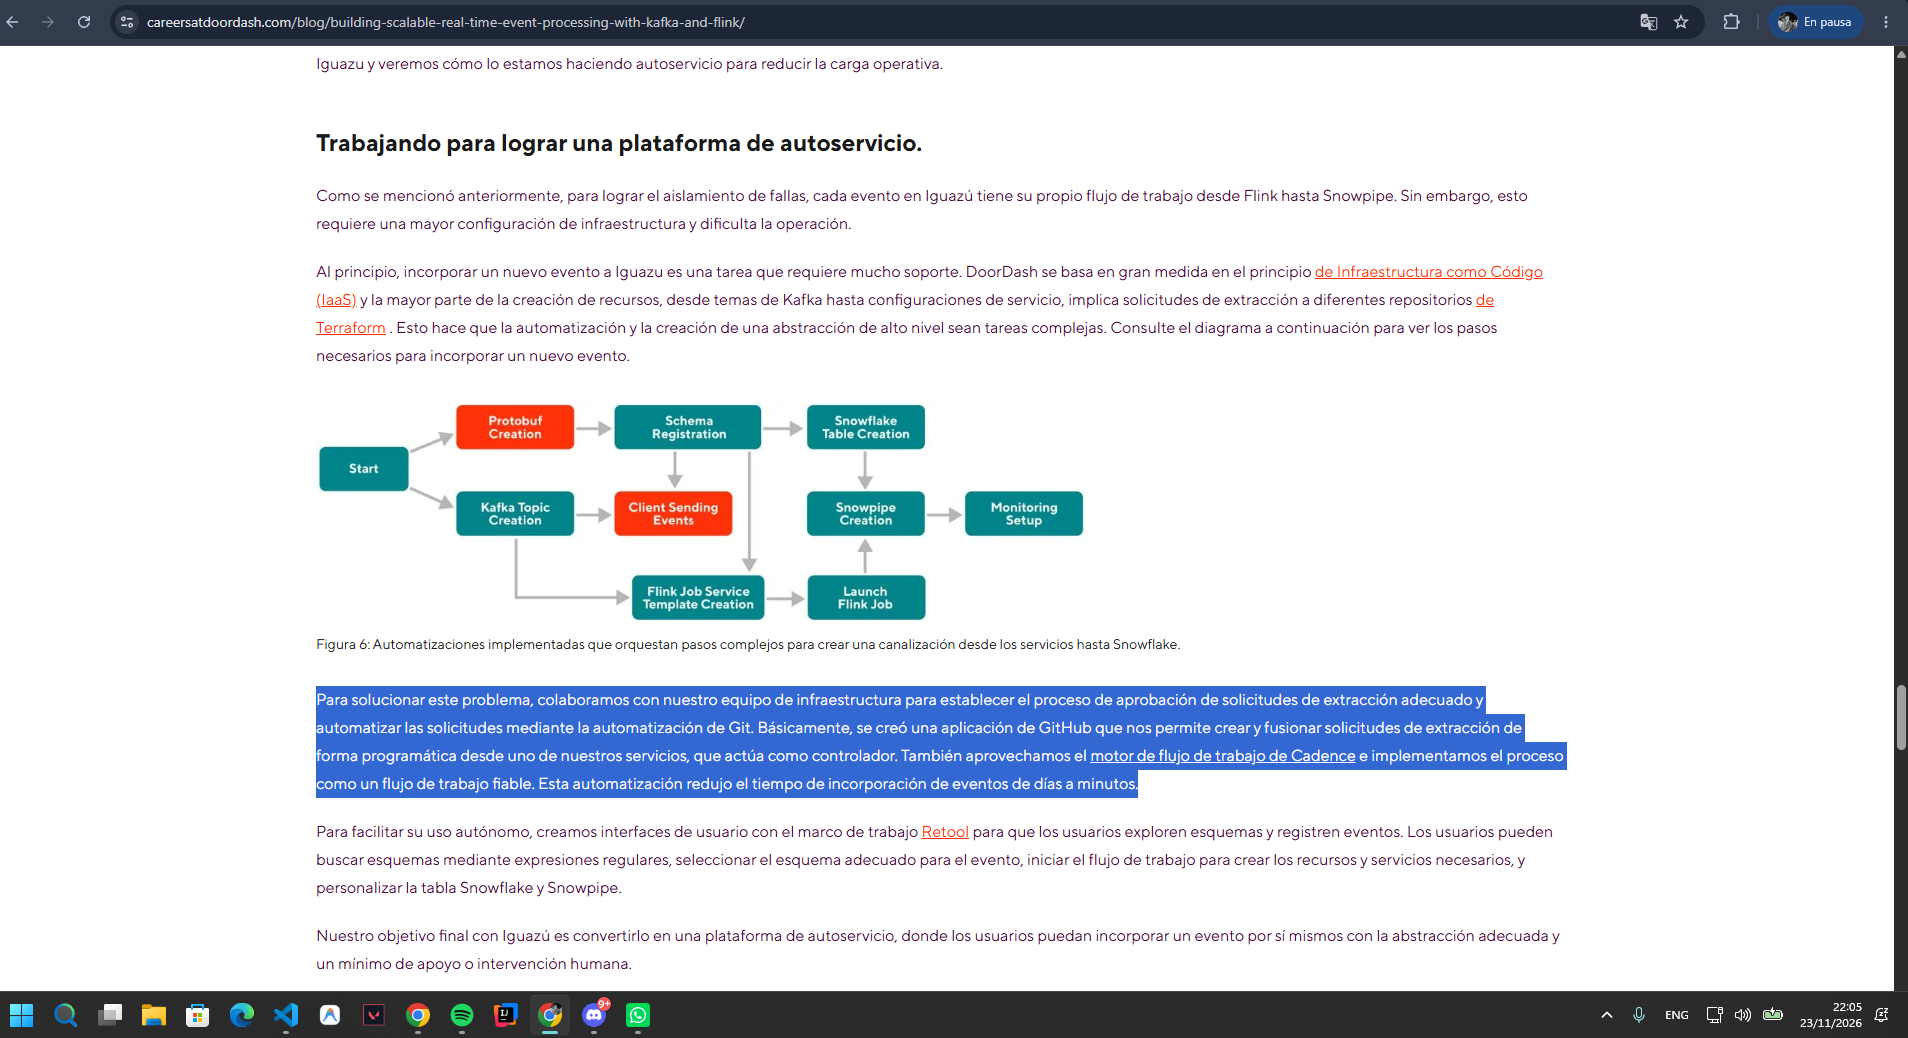
\includegraphics[width=0.95\textwidth]
    {evidencias/05_automatizacion_eventos.png}
    \caption{Automatización del proceso de incorporación
    de nuevos eventos mediante GitHub y Cadence.}
    \label{fig:automatizacion-eventos}
\end{figure}

\subsection*{A.2. Ejemplo conocido de primera mano}

Durante la preparación de la exposición GA-SUM-01 de Aplicaciones Distribuidas, realicé una práctica del patrón Publish/Subscribe utilizando el protocolo MQTT y Eclipse Mosquitto, tomando como contexto el Sistema de Gestión de Refuerzo Académico (SGRA).

En la demostración, un publicador enviaba un mensaje al tópico \texttt{sgra/tutorias/creada}, mientras que dos suscriptores, que representaban los componentes de notificaciones y auditoría, recibían el mismo mensaje de forma independiente.

También se realizó una prueba con Java y Spring Boot, utilizando un publicador MQTT conectado a un broker Mosquitto real y simulando el repositorio de datos mediante Mockito.

Esta experiencia permitió reconocer el desacoplamiento entre productores y consumidores, principio presente en la arquitectura de Iguazu. Aunque la práctica no constituye una implementación completa de EDA en producción, demuestra su mecanismo de comunicación mediante eventos.

\subsection*{A.3. Declaración de uso de inteligencia artificial}

Para el desarrollo de esta actividad se utilizó ChatGPT de OpenAI (modelo GPT-6.2 en la sesión consultada) como herramienta de apoyo para la organización del trabajo, comprensión de conceptos arquitectónicos y estructuración del documento en LaTeX (ayuda con comandos que desconozco).
